\documentclass{report}
\usepackage{hyperref}
\usepackage{geometry}
\usepackage{scalerel,amssymb}
\usepackage{paralist}
\usepackage{colortbl}
\usepackage{amsmath}
\usepackage{pgfplots}
\usepackage{xcolor}
\usepackage{tikz}
\usetikzlibrary{positioning}
\usetikzlibrary{shapes.geometric, arrows}
\tikzstyle{arrow} = [thick,->,>=stealth]

\usepackage{stackengine}
\def\apeqA{\SavedStyle\sim}
\def\apeq{\setstackgap{L}{\dimexpr.5pt+1.5\LMpt}\ensurestackMath{%
  \ThisStyle{\mathrel{\Centerstack{{\apeqA} {\apeqA} {\apeqA}}}}}}

\begin{document}
\begin{center}
\huge{\textbf{\underline{Cryptography}}}
\end{center}

	{\let\clearpage\relax \chapter*{7 Security against chosen-plaintext attacks}}
	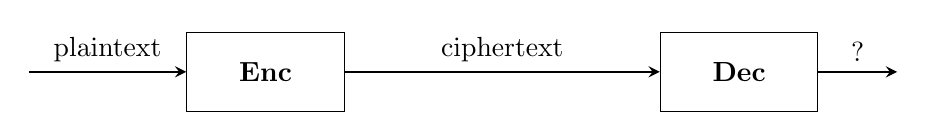
\begin{tikzpicture}
							\coordinate (start);
							
							%Nodes
							\node (rect) [draw,thin,minimum width=2cm,minimum height=1cm, right=2cm of start] (Enc) {\textsc{\textbf{Enc}}};
							\node (rect) [draw,thin,minimum width=2cm,minimum height=1cm, right=4cm of Enc] (Dec) {\textsc{\textbf{Dec}}};
							\node [right=of Dec] (stop) {};
							
							%Lines
							\draw[arrow] (start) -- node[ anchor=south ]{plaintext} (Enc.west);
							\draw[arrow] (Enc.east) -- node[ anchor=south ]{ciphertext} (Dec.west);
							\draw[arrow] (Dec.east) -- node[ anchor=south ]{?} (stop.west);
							
	\end{tikzpicture} \\
	\begin{tabular}{lll}
		\begin{tabular}{l}
			increasing adversary power
		\end{tabular}
		&
		\begin{tabular}{l}
			$\downarrow$
			\end{tabular}
		&
		\begin{tabular}{l}
			known-plaintext \\
			chosen-plaintext {\LARGE{ $\rbrace$ }} attack\\	
			chosen ciphertext
		\end{tabular}
	\end{tabular} \\
	\underline{One-time security}
	\begin{enumerate}[-]
		\item not very useful
		\item chooses a fresh key per encryption cell \\
		$\Rightarrow$ relax this!
	\end{enumerate}
	\subsection*{Definition}
		A encryption scheme $\Sigma$ is secure against chosen-plaintext attacks if $L_{cpa-L}^{\Sigma} \apeq L_{cpa-R}^{\Sigma}$, where: \\ \\
		\begin{tabular}{lll}
			\begin{tabular}{|l|}
				\hline \underline{$L_{cpa-L}^{\Sigma}$} \\
				$ \ k \leftarrow \{ 0,1 \} ^{\lambda}$ \\
				\\
				\ \underline{\textsc{Eavesdrop}($m_L, m_R$)} \\
				\ \ \underline{if} $\mid m_L \mid \ \neq \ \mid m_R \mid$ \\
				\ \ \underline{then} return \textsc{Error} \\
				$ \ \ c := \Sigma.Enc(k, m_L)$ \\
				\ \ return c \\ \hline
				\end{tabular}
			&
			&
			\begin{tabular}{|l|}
				\hline \underline{$L_{cpa-R}^{\Sigma}$} \\
				$ \ k \leftarrow \{ 0,1 \} ^{\lambda}$ \\
				\\
				\ \underline{\textsc{Eavesdrop}($m_L, m_R$)} \\
				\ \ \underline{if} $\mid m_L \mid \ \neq \ \mid m_R \mid$ \\
				\ \ \underline{then} return \textsc{Error} \\
				$ \ \ c := \Sigma.Enc(k, m_R)$ \\
				\ \ return c \\ \hline
			\end{tabular}
		\end{tabular}
		\begin{enumerate}[NOTE 1:]
			\item Lengths must be equal. That allows $\Sigma$ to be used for plaintext of different lengths: \\
			$\Sigma.M \ = \ \{ 0,1 \} ^{\star}, \ \ \ \mid m \mid \ = \ length \ in \ bits$
			\begin{enumerate}[\textbullet]
				\item Traffic analysis reveals information about plaintext sizes
				\item Steganography hides the existence of a hidden message
			\end{enumerate}
			\item Often called IND-CPA security (indistinguishable CPA)
			\item Almost same notion for public key crypto.
		\end{enumerate}
	 \subsection*{Lemma}
	 CPA-secure encryption schemes cannot be deterministic.
	 \subsection*{Proof}
	 \textit{Suppose it is:} \\
	 Then: 
	 \begin{align*}
	 	& c_x := EAVESDROP(x,x); \\
	 	& c_y := EAVESDROP(x,y); \\
	 	& \textbf{return} \ c_x \stackrel{?}{=} c_y
	 \end{align*}
	 distinguishes between $L_{cpa-L}^{\Sigma}$ and $L_{cpa-R}^{\Sigma}$. \\
	 \textit{\textbf{Need probabilistic encryption!}}
	 \subsubsection*{\underline{How to make encryption non-deterministic?}}
	 \begin{enumerate}
	 	\item \underline{Stateful encryption}
	 	\begin{enumerate}[-]
	 		\item Keep state (counter) inside $\Sigma$.Enc()
	 		\item Complex to implement: \\
	 		requires synchronisation between Enc() and Dec()
	 	\end{enumerate}
	 	\item \underline{Randomization in encryption algorithm}
	 	\begin{enumerate}[-]
	 		\item $\Sigma$.Enc uses randomness $r$
	 		\item $r$ becomes part of ciphertext: \\
	 		$\Rightarrow$ increases length
	 		\item most popular
	 	\end{enumerate}
	 	\item \underline{Nonce-based encryption}
	 	\begin{enumerate}[-]
	 		\item add a nonce to $\Sigma$.Enc()
	 		\item nonce: number used once
	 		\item caller must ensure that Enc() is never called with the same nonce twice
	 	\end{enumerate}
	 \end{enumerate}
	 \subsection*{Pseudorandom ciphertext}
	 \begin{enumerate}
	 	\item Second notion for CPA-secure symmetric encryption
	 	\item Often more useful than CPA
	 \end{enumerate}
	 \subsection*{Definition}
	 An encryption scheme $\Sigma$ has pseudorandom ciphertexts against chosen-plaintext attacks if \\
	 $L_{cpa\$-real}^{\Sigma} \apeq L_{cpa\$-rand}^{\Sigma}$ \\
	 \begin{tabular}{lll}
			\begin{tabular}{|l|}
				\hline \underline{$L_{cpa\$-real}^{\Sigma}$} \\
				$ \ k \leftarrow \{ 0,1 \} ^{\lambda}$ \\
				\\
				\ \underline{\textsc{CTxt}($m$)} \\
				$ \ \ c := \Sigma.Enc(k, m)$ \\
				\ \ return c \\ \hline
				\end{tabular}
			&
			&
			\begin{tabular}{|l|}
				\hline \underline{$L_{cpa\$-rand}^{\Sigma}$} \\
				\\
				\ \underline{\textsc{CTxt}($m_L, m_R$)} \\
				$ \ \ r \leftarrow \Sigma.C \mid _{length(r) = length(\Sigma.Enc(k,m))}$ \\
				\ \ return r \\ \hline
			\end{tabular}
		\end{tabular}
	 \subsection*{Lemma}
	 	CPA\$-security $\Rightarrow$ CPA-security ($\nLeftarrow$)
	 \subsection*{Proof}
	 	Exercise
	 \subsection*{CPA-secure encryption from a PRF}
	 	\underline{Idea:} Use $F(k,r)$ with a different $r$ for each encryption call. \\
	 	\underline{How to make $r$ distinct?} \\
	 	\begin{enumerate}[-]
	 		\item statful encryption: $r$: counter/state, complex
	 		\item Randomized: $r \leftarrow \{ 0,1 \} ^{\lambda}$
	 		\item Delegate it: use nonce, $r \ := \ nonce$
	 	\end{enumerate}
	 \subsection*{Construction:}
	 CPA-secure $\Sigma$ from PRF $F$
	 \[
	 	F: \{ 0,1 \}^{\lambda} \times \{ 0,1 \} ^{\lambda} \rightarrow \{ 0,1 \} ^{len}
	 \]
	 \begin{tabular}{lll}
	 	\begin{tabular}{l}
	 		$\Sigma.M \ = \ \{ 0,1 \} ^{\lambda}$ \\
	 		$ \Sigma.C \ = \ \{ 0,1 \}^{\lambda} \times \{ 0,1 \} ^{len}$ \\
	 		$\Sigma.K \ = \ \{ 0,1 \} ^{\lambda}$
	 	\end{tabular}
	 	&
	 	&
	 	\begin{tabular}{l}
	 		\underline{KeyGen():} \\
	 		\ $k \leftarrow \{ 0,1 \} ^{\lambda}$ \\
	 		\ \textbf{return} $k$
	 	\end{tabular}
	 \end{tabular}
	 \\ \\ \\
	 \begin{tabular}{lll}
	 	\begin{tabular}{l}
	 		\underline{$\Sigma$.Enc(k,m):} \\
	 		\ $r \leftarrow \{ 0,1 \} ^{\lambda}$ \\
	 		\ $x := F(k,r) \oplus m$ \\
	 		\ \textbf{return} F(r,x)
	 	\end{tabular}
	 	&
	 	&
	 	\begin{tabular}{l}
	 		\underline{$\Sigma$.Dec(r,x):} \\
	 		\ \textbf{return} $F(k,r) \oplus x$
	 	\end{tabular}
	 \end{tabular}
	 \subsection*{Lemma}
	 If F use a secure PRF then construction has CPA\$-security.
	 \subsection*{Proof idea}
	 \begin{tabular}{lll}
	 	\begin{tabular}{|l|}
	 		\hline \underline{$L_{cpa\$-real}^{\Sigma}$} \\
	 		$ \ k \leftarrow \{ 0,1 \} ^{\lambda}$ \\
			\\
			\ \underline{\textsc{CTxt}($m$)} \\
			\ \ $ r \leftarrow \{ 0,1 \} ^{\lambda}$ \\
			\ \ $x := F(k,r) \oplus m$ \\
			\ \ \textbf{return} $(r,x)$ \\ \hline
		\end{tabular}
	 	&
	 	&
	 	\begin{tabular}{|l|}
	 		\hline \underline{$L_{cpa\$-rand}^{\Sigma}$} \\
	 		\ $ r \leftarrow \{ 0,1 \} ^{\lambda}$ \\
	 		\ $ x \leftarrow \{ 0,1 \} ^{len}$ \\
	 		\ \textbf{return} $(r,x)$ \\ \hline
	 	\end{tabular}
	 \end{tabular}
	 \chapter*{8 Block ciphers in practice}
	 \begin{enumerate}[\textbullet]
	 	\item Blockcipher as a PRP
	 	\item How to encrypt \underline{long} messages?
	 \end{enumerate}
	 \begin{enumerate}[\textbullet]
	 	\item \textbf{\underline{Mode of operation}} \\
	 	Needed to implement CPA-secure encryption of long messages.
	 	\item \textbf{\underline{Padding scheme}}
	 \end{enumerate}
\end{document}
 